272. Заметим, что кубик может попасть на ту же грань, на которой стоял, минимум через 3 перекатывания, значит испачкать можно максимум треть клеток, то есть $3\cdot5:3=5.$ На картинке приведён один из возможных вариантов это сделать. Испачканной выберем ту грань, которая стоит на клетках 2, 5, 8, 11, 14.
\begin{center}
\begin{figure}[ht!]
\center{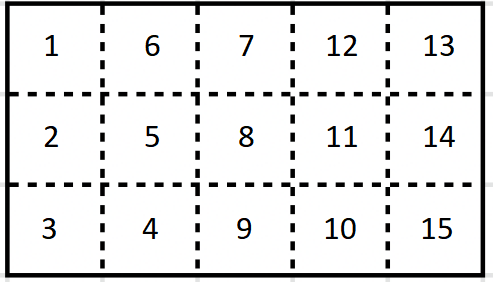
\includegraphics[scale=0.35]{kub1s.png}}
\end{figure}
\end{center}
\newpage\noindent
